\documentclass[aps,physrev,10pt,floatfix,reprint]{revtex4-2}

\usepackage{graphicx}% Include figure files
\usepackage{dcolumn}% Align table columns on decimal point
\usepackage{bm}% bold math
\usepackage{hyperref}% add hypertext capabilities
\usepackage[mathlines]{lineno}% Enable numbering of text and display math
%\linenumbers\relax % Commence numbering lines

\usepackage[%Uncomment any one of the following lines to test 
scale=0.7, marginratio={1:1, 2:3}, ignoreall,% default settings
text={7in,10in},centering,
%%margin=1.5in,
%%total={6.5in,8.75in}, top=1.2in, left=0.9in, includefoot,
%%height=10in,a5paper,hmargin={3cm,0.8in},
]{geometry}
\usepackage[utf8]{inputenc}
\usepackage{amsmath}
\usepackage{amstext}
\usepackage{graphicx}
\usepackage{esint}
\usepackage{geometry}
\usepackage{hyperref}
\usepackage{amsfonts}

\hypersetup{
    colorlinks=true,
    linkcolor=blue,
    filecolor=magenta,      
    urlcolor=cyan,
    pdftitle={Overleaf Example},
    pdfpagemode=FullScreen,
    }
%\geometry{verbose,lmargin=2cm,rmargin=2cm}

\begin{document}

%\title{Autoregressive neural network of spins system: the deepness of Mean-Field models}
\title{Autoregressive neural network architecture of the Boltzmann distribution: the cases of two body interacting systems and two mean-field models.}
\author{Biazzo, Indaco}
 \altaffiliation[Also at ]{Physics Department, XYZ University.}
 %Lines break automatically or can be forced with \\
\date{\today}

\begin{abstract}
    Generative neural networks received, in recent years, increasing attention from both scientific and private domains. Generative autoregressive transformers, particularly, incredibly improves previous performances in image and language generative tasks. To gain physical intuition about generative Autoregressive Neural Network (ANN) architectures, this work rewrites the Boltzmann distribution of a generic pairwise interacting binary variables hamiltonian as a generative neural network in the autoregressive form. The result is a deep ANN architecture with weights and biases of the first layer corresponding to couplings and external fields of the Hamiltonian, respectively, featuring properties, commonly used in the computer science literature, such as residual connections and recurrent structures but now with clear physical interpretations. However, one of their hidden layers grows exponentially with system size, making their use impractical for realistic scenarios. To address this issue, ANN architectures for two paradigmatic mean-field statistical physics systems - Curie-Weiss (CW) model and Sherrington-Kirkpatrick (SK) model - are derived. The exact ANN architecture of the CW model is derived at finite numbers of variables and in the thermodynamic limit, resulting in deep architectures with parameters that scale polynomially with system size. For the SK model, an approximate ANN architecture is derived relying on k-step replica symmetric breaking (k-RSB) ansatz of the Parisi solution; transforming its exponentially large hidden layer into a deep structure where every step of replica symmetric breaking corresponds to adding a linear layer and a non-linear operator. The number of parameters scales polynomially with system size at finite k-RSB. The derived architectures are tested against other ANN architectures with an equivalent number of parameters for CW and SK models, showing superior performance over large regions of physical phase space. This general framework allows using statistical physics approaches to derive new ANN architecture for different interacting systems and interpret existing ones from a physical perspective.    \\
    \textbf{Keywords:} Autoregressive neural network, Generative model, Statistical physics, Machine learning, Deep learning, Mean field model, Curie-Weiss model, Sherrington-Kirkpatrick model.  
\end{abstract}
    
    %\keywords{Suggested keywords}%Use showkeys class option if keyword
                                  %display desired
    
\maketitle
\tableofcontents
\section{Introduction}
The cross fertilization among machine learning and statistical physics continues for decades.
In particular, the development of deep neural network frameworks \cite{bengioNatureDeepLearning2015} have been applied to a long list of statistical physics problems \cite{RevModPhys.91.045002} spanning a wide range of domains, including quantum mechanics \cite{doi:10.1126/science.aag2302}, 
classical statistical physics, chemical and biological physics \cite{noe2019boltzmann,jumper2021highly}, and complex inference problems.
On the other hand, techniques borrowed from statistical physics have been used to shed light on the behavior of Machine Learning algorithms.
Talk about generative models and transformers. \\
In this work, neural network architectures of the Boltzmann distribution of statistical physics models are derived, specifically in the context of generative models.
Here, I focus on classical spin systems with pairwise interacting Hamiltonians. These systems are commonly studied in statistical physics, and the goal is to show how to derive autoregressive neural network architectures directly from the system Hamiltonian. Autoregressive models are a type of generative model that predicts the next element in a sequence given all previous elements. In our case, the sequence is a subset of the configuration of spins of the system, and the goal of the model is to learn to generate new configurations that are likely according to the Hamiltonian. By deriving the neural network architecture from the Hamiltonian, we can establish a direct link between the parameters of the Hamiltonian and the parameters of the neural network.\\
In general, ANN architectures for these systems tend to involve an exponential growth in the number of parameters with the number of spins in the system. However, we derive new architectures for two mean-field models, namely the Curie-Weiss model and the Sherrington-Kirkpatrick model, where the number of parameters scales polynomially with the number of spins. This is a significant improvement, as it allows for the scalability of the model to large systems. Our derived architecture also shares several interesting properties with commonly used architectures, such as being deep, having residual and skip connections, being recurrent by construction, and being able to learn the Hamiltonian parameters. Additionally, the parameters of the first layer of the network are directly related to the Hamiltonian parameters and are shared among all the spins, which allows to take advantage of the underlying symmetry of the problem to learn more efficiently.\\
            

%\section{Materials and Methods}
\section{Pair-wise Ising model in autoregressive conditional probability form}
Consider a generic Hamiltonian $H[\mathbf{x}]$ that depends on a set of $N$ binary variables $\mathbf{x}=\{x_1, x_2,...x_N\}$. The Boltzmann distribution at inverse temperature $\beta$ is:
\begin{equation}
P\left(\mathbf{x}\right)=\frac{e^{-\beta H\left(\mathbf{x}\right)}}{\sum_{\left\{ x\right\} }e^{-\beta H\left(\mathbf{x}\right)}}.
\end{equation}
It is generally challenging to compute marginals and average quantities when $N$ is large, and sampling from these distributions is difficult on frustrated systems. I defined the sets of variables $\mathbf{x}_{<i}=\left(x_{1},x_{2}\dots x_{i-1}\right)$ and $\mathbf{x}_{>i}=\left(x_{i+1},x_{i+2}\dots x_{N}\right)$ respectively with an index lower and larger than $i$, then if we can rewrite the Boltzmann distribution in the autoregressive form:
\begin{equation}
P\left(\mathbf{x}\right)=\prod_{i}P\left(x_{i}|\mathbf{x}_{<i}\right)
\end{equation}
then it would be straightforward to produce independent samples from it, thanks to the ancestral sampling procedure. It has been proposed to use a variational approach to approximate the Boltzmann distribution with trial probability distributions that have this autoregressive form where each conditional probability is represented by a feed-forward neural network with a set of parameters ${\theta}$:
\begin{equation}
Q^{\theta}\left(\mathbf{x}\right)=\prod_{i}Q^{\theta_i}\left(x_{i}|\mathbf{x}_{<i}\right)
\end{equation}
The parameters ${\theta}$ can be learn minimizing the Kullback-Leibler divergence $D_{KL}$,
with the true probability function:
\begin{equation}
\begin{split}
& D_{KL}\left(P|Q^{\Theta}\right) =  \sum_{\left\{ x\right\} }Q^{\Theta}\left(\mathbf{x} \right)\ln\left(\frac{Q^{\Theta}\left(\mathbf{x} \right)}{P\left(\mathbf{x} \right)}\right)  \\
& \approx \sum_{\mathbf{x}\sim Q^{\Theta}}\left[\ln\left(Q^{\Theta}\left(\mathbf{x} \right)\right)-\ln\left(P\left(\mathbf{x} \right)\right)\right]
\end{split}    
\end{equation}
Thanks to the ancestral sampling, we substituted the sum over all possible configurations with a subset of configurations extracted from the autoregressive trial functions.
In this framework, the choice of the architecture of the neural networks is crucial.
In this work, we want to find neural network architectures that can represent solvable mean-field statistical physics systems. 
Then, these architectures could be used as an {\it ansatz} for more complex systems or in different limits (for instance, at finite $N$).


\subsection{Conditionals}
 We want to find a form of a generic $i$-th conditional probability factor of the Boltzmann distribution as a feed-forward neural network. First, we can rewrite a generic conditional in this form: 
\begin{equation}
    \label{eq:chain}
    \begin{split}
    & P\left(x_{i}|\mathbf{x}_{<i}\right)  = 
    \frac{P\left(\mathbf{x}_{<i+1}\right)}{P\left(\mathbf{x}_{<i}\right)}  = 
    \frac{\sum_{\mathbf{x}_{>i}}P\left(\mathbf{x}\right)}{\sum_{\mathbf{x}_{>i-1}}P\left(\mathbf{x}\right)} \\
    &=\frac{\sum_{\mathbf{x}_{>i}}e^{-\beta H}}{\sum_{\mathbf{x}_{>i-1}}e^{-\beta H}}  = 
    \frac{f\left(x_{i},\mathbf{x}_{<i}\right)}{\sum_{x_{i}}f\left(x_{i},\mathbf{x}_{<i}\right)}.
    \end{split}
\end{equation}
where I defined: $f\left(x_{i}=\pm 1,\mathbf{x}_{<i}\right) = \sum_{x_{i+1}\dots x_{N}}e^{-\beta H}\delta_{x_i, \pm1}$. Usually, in the representation of the conditional probability $P\left(x_{i}=1|\mathbf{x}_{<i}\right)$ as a feed-forward neural network, the set of variable $\mathbf{x}_{<i}$ is the input, and the sigma function $\sigma(x)=\frac{1}{1+e^{-x}}$ is the last layer, assuring that the output is between $0$ and $1$. The probability $P\left(x_{i}=-1|\mathbf{x}_{<i}\right) = 1 - P\left(x_{i}=1|\mathbf{x}_{<i}\right)$ is straightforward to obtain. With simple algebraic manipulations, we can write: 
\begin{equation}
    \label{eq:sigma_log}
    \begin{split}
    & P\left(x_{i}=1|\mathbf{x}_{<i}\right) = \frac{f\left(1,\mathbf{x}_{<i}\right)}{\sum_{x_{i}}f\left(x_{i},\mathbf{x}_{<i}\right)}\\
    &= \sigma\left(\log\left[f\left(1,\mathbf{x}_{<i}\right)\right]-\log\left[f\left(-1,\mathbf{x}_{<i}\right)\right]\right)
    \end{split}
\end{equation}
Consider a generic two-body interaction Hamiltonian of binary spin variables $x_i \in \{-1,1\}$, $H = -\sum_{i<j} J_{ij} x_i x_j - \sum_{i} h_i x_i$, where $J_{ij}$ are the interaction couplings and $h_i$ are the external fields. Substituting it in eq.\ref{eq:sigma_log}, we obtain:
\begin{figure}[!ht]
    %\centering 
    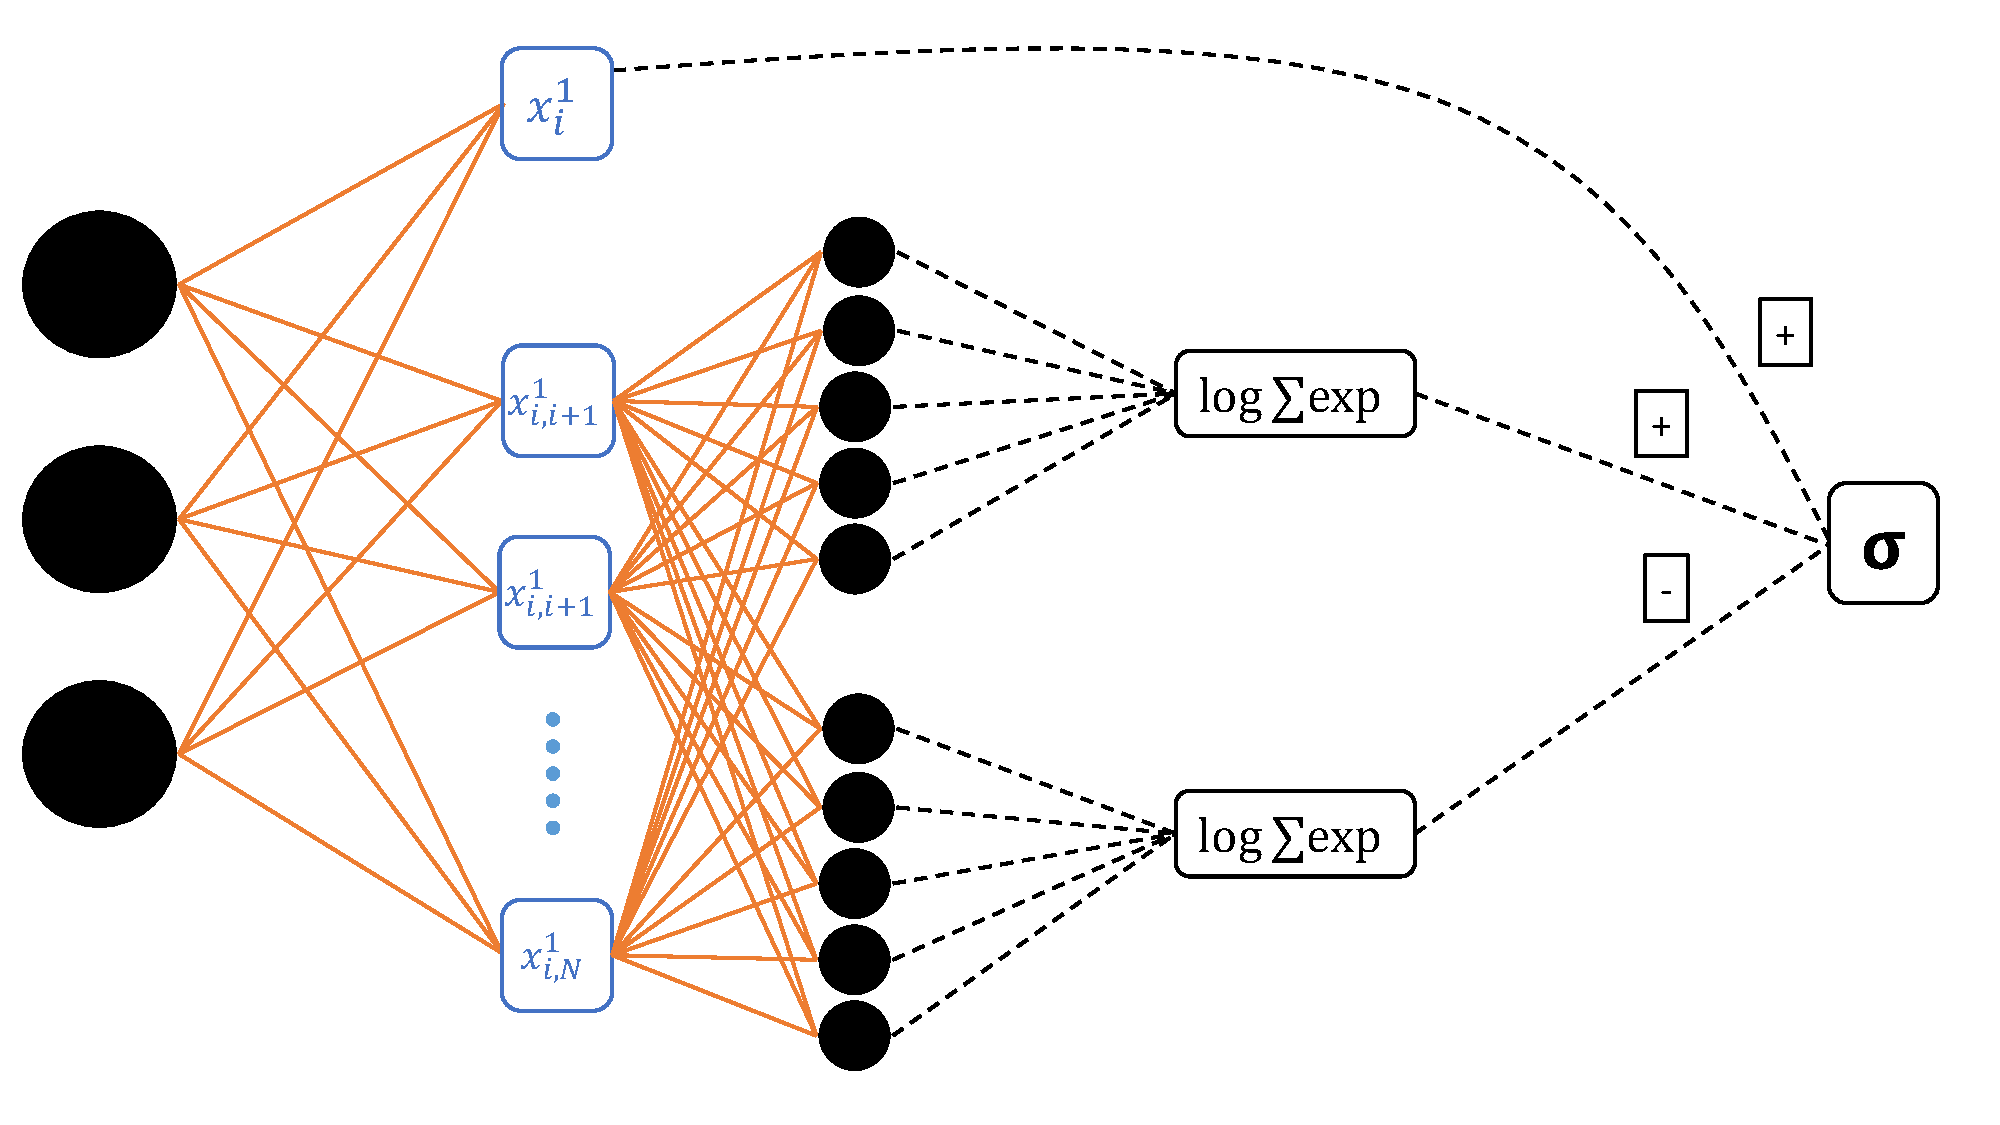
\includegraphics[width=0.45\textwidth]{img/twoboghann.pdf}
    \caption{Neural network Architectures of conditional probability}
    \label{fig:arch}
\end{figure}
\begin{equation}
    \label{eq:conditional_ghann}
    \begin{split}
    & P\left(x_{i}=1|\mathbf{x}_{<i}\right) = \\
    & \sigma\left( 2 \beta \left(h_i + \sum_{s=1}^{i-1} J_{si} x_s\right) +\log(\rho_i^+) - \log(\rho_i^-)
    \right),   
    \end{split}
\end{equation}
where:
\begin{equation}
    \begin{split}
    \rho_i^{\pm}&[\mathbf{x}_{<i}]  = \sum_{\mathbf{x}_{>i}}  \exp \bigg(
    \beta\sum_{l=i+1}^{N} x_l \sum_{s=1}^{i-1} J_{sl} x_s +\\
    &\beta\sum_{l=i+1}^{N}\big( \pm J_{il}  + h_l \big) x_l 
    + \beta\sum_{l=i+1}^{N}\sum_{l'=l+1}^{N} J_{ll'} x_l x_{l'} \bigg)
\end{split}
\label{eq:rho_ghann}
\end{equation}
The elements in $H$ that depend only on s$\mathbf{x}_{<i}$ cancel out.
The conditional probability, eq.\ref{eq:conditional_ghann}, can be interpreted as a feed-forward neural network, with the following architecture (see fig.\ref{fig:arch}) :
\begin{multline}
     Q^{\theta}\left(\mathbf{x}_{<i}\right) = 
     \sigma \bigg\{ x_i^1(\mathbf{x}_{<i})+\log\big[ \sum_{c} e^{b_c^+ + \sum_{l=i+1}^{N} w_{cl} x_{il}^1(\mathbf{x}_{<i})}\big] \\
     +\log\big[ \sum_{c} e^{b_c^- + \sum_{l=i+1}^{N} w_{cl} x_{il}^1(\mathbf{x}_{<i})}\big] \bigg\},
\end{multline}
where $x_i^1(\mathbf{x}_{<i})=\sum_{s=1}^{i-1} J_{si} x_s$ and $x_{il}^1=\sum_{s=1}^{i-1} J_{sl} x_s$ are the output of the first layer. 
Then, a second layer acts on the set of $x_{il}^1$ (see fig.\ref{fig:arch}). The $\sum_{c}$ is over the $2^{N-i}$ number of configurations of the set of $\mathbf{x}_{>i}$ variables. 
The parameters of the second layers are the $b_c^{\pm} = \beta\sum_{l=i+1}^N (\pm J_{il} + h_l + \sum_{l'=l+1}^N J_{ll'}x_{l'}) x_l $ and the $w_{cl}=x_l$, where $c$ is the index of the configuration of the set of $\mathbf{x}_{>i}$ variables. Then, the two functions $\rho^{\pm}$ are obtained by applying the non-linear operator $f(\mathbf{x}) = \log(\sum_i e^{x_i})$ at the output of the second layer (see fig.\ref{fig:arch}). 
As the last layer, the two $\rho^{\pm}$ and $x_i^1$ are summed, and the sigma function is applied. The whole architecture of the Boltzmann distribution of a 2-BOdy General Hamiltonian of an Autoregressive Neural Network (2BoGHANN) is depicted in fig.\ref{fig:arch}. The total number of parameters scales exponentially with the system size, making the sampling infeasible after a few spins.
 Nevertheless, the 2BoGHANN architecture shows some interesting futures:
\begin{itemize}
    \item As for the author known, it is the first time that a neural network architecture is proposed to represent the autoregressive Boltzmann probability distribution of a classical physical system where the weights and biases of the first layers are the parameters of the Hamiltonian. In this case, its couplings and fields. 
    \item Residual connections among layers, due to the $x_i^1$ variables, naturally emerge from the derivation. 
    The extensive use of residual connections in recent \cite{10.48550/arxiv.1512.03385}, but became quickly a central element in the success of the ResNet and transformer architectures \cite{vaswani2017attention}, in classification and generative tasks. They were presented as a way to improve the training of deep neural networks avoiding the exploding and vanishing gradient problem. In our context, they represent the direct interactions among the variable $x_i$ and all the previous variables $\mathbf{x}_{<i}$. 
    On the other hand, the functions $\rho_i^{\pm}$ take into account the effect of the interactions among $\mathbf{x}_{<i}$ and $\mathbf{x}_{>i}$ on the variable $x_i$, and needs an exponential number of parameters in the feed-forward representation in the general case. 
    %This distinctions of clearly identification of the porpouse of the elements in the architecture of the neurla could help shed light on the nature of residual connections in neural network architectures. 
    \item Since the starting of teh deep learning revolution the recurrent neural network had central role. that some NN architecture that deal with autoregressive problems is the recursive architecture of the neural network \cite{bengioNatureDeepLearning2015}. 
    For instance, in \cite{10.1038/s42256-021-00401-3} a recursive autoregressive neural network is used to find the zero temperature configurations of spin glass systems. 
    It is easy to show that also the 2BoGHANN encodes a recursive structure. 
    Consider the first layer of the 2BoGHANN, see figure \ref{fig:arch}. The first layer is composed of the following set of linear operators on the input $x_{il}(\mathbf{x}_{<i})=\sum_{s=1}^{i-1} J_{si} x_s$ and $\omega_{il}=\sum_{s=1}^{i-1} J_{sl} x_s$ with $i<l<=N$. 
    The set of $\omega_{il}$ can be rewritten in recursive form observing that:
    \begin{equation}
    \omega_{il} = \omega_{i-1,l} + J_{i-1,l} x_{i-1}
    \end{equation}
    The neurons $\omega_{il}$ in the first layer of each conditional probability in the 2BoGHANN architecture depend on the $\omega_{i-1,l}$ of the previous conditional probability, lighting up the recurrent nature of the 2BoGHANN architecture.
\end{itemize}

%This dependence on the size of the system appears reasonable because, otherwise, it could be possible to sample to whatever pairwise hamiltonian in polynomial time, and as long we assume that $P\neq NP$ it could not be possible. 
%The computational cost of the sum over all the configuration of spins $x_l$ grows exponentially with the system's size making it unfeasible, after a few spins, the explicit computations. The idea is to find feed-forward neural network architectures representing these functions with a polynomial number of free parameters. \\
The challenge is to find simplified neural network representations of the $\rho_i^{\pm}$ functions, eq.\ref{eq:rho_ghann}. Closely looking, they can be seen very similar to the partition function of the system, where the variables are $\mathbf{x}_{>i}$ and the fixed values of the variables $x_{<i}$ act like external fields.
In the following, I show how to use technics derived for solving statistical mechanics systems to construct neural networks based on the physical solution of pairwise interaction systems. In particular, neural network architectures for two exact solvable models: the Curie-Weiss model (CW) and the Sherrington-Kirkpatrick model (SK) in the thermodynamical limit, will be derived. These fully connected models are chosen due to their paradigmatic role in the history of statistical physics systems. The CW model, despite its straightforward hamiltonian, displays a second-order phase transition and, as shown after, has a deep architecture that scales as $O(N^2)$ to be sampled exactly at finite N. The SK model was one of the first models to describe the behavior of spin glasses successfully, and it provided a theoretical framework for understanding the complex behavior of these materials. The SK model is a mean-field model and it can be solved analytically \cite{}, thanks to the celebrated replica symmetric breaking solutions of Parisi. The complex and universal(?) landscape of the SK model at low temperatures that emerge from the solutions [cite] allowed to apply the idea and the replica computations in very different domains, like computer science [cite], statistical inference problems, and biology. \\

\begin{figure}[!h]
    \centering 
    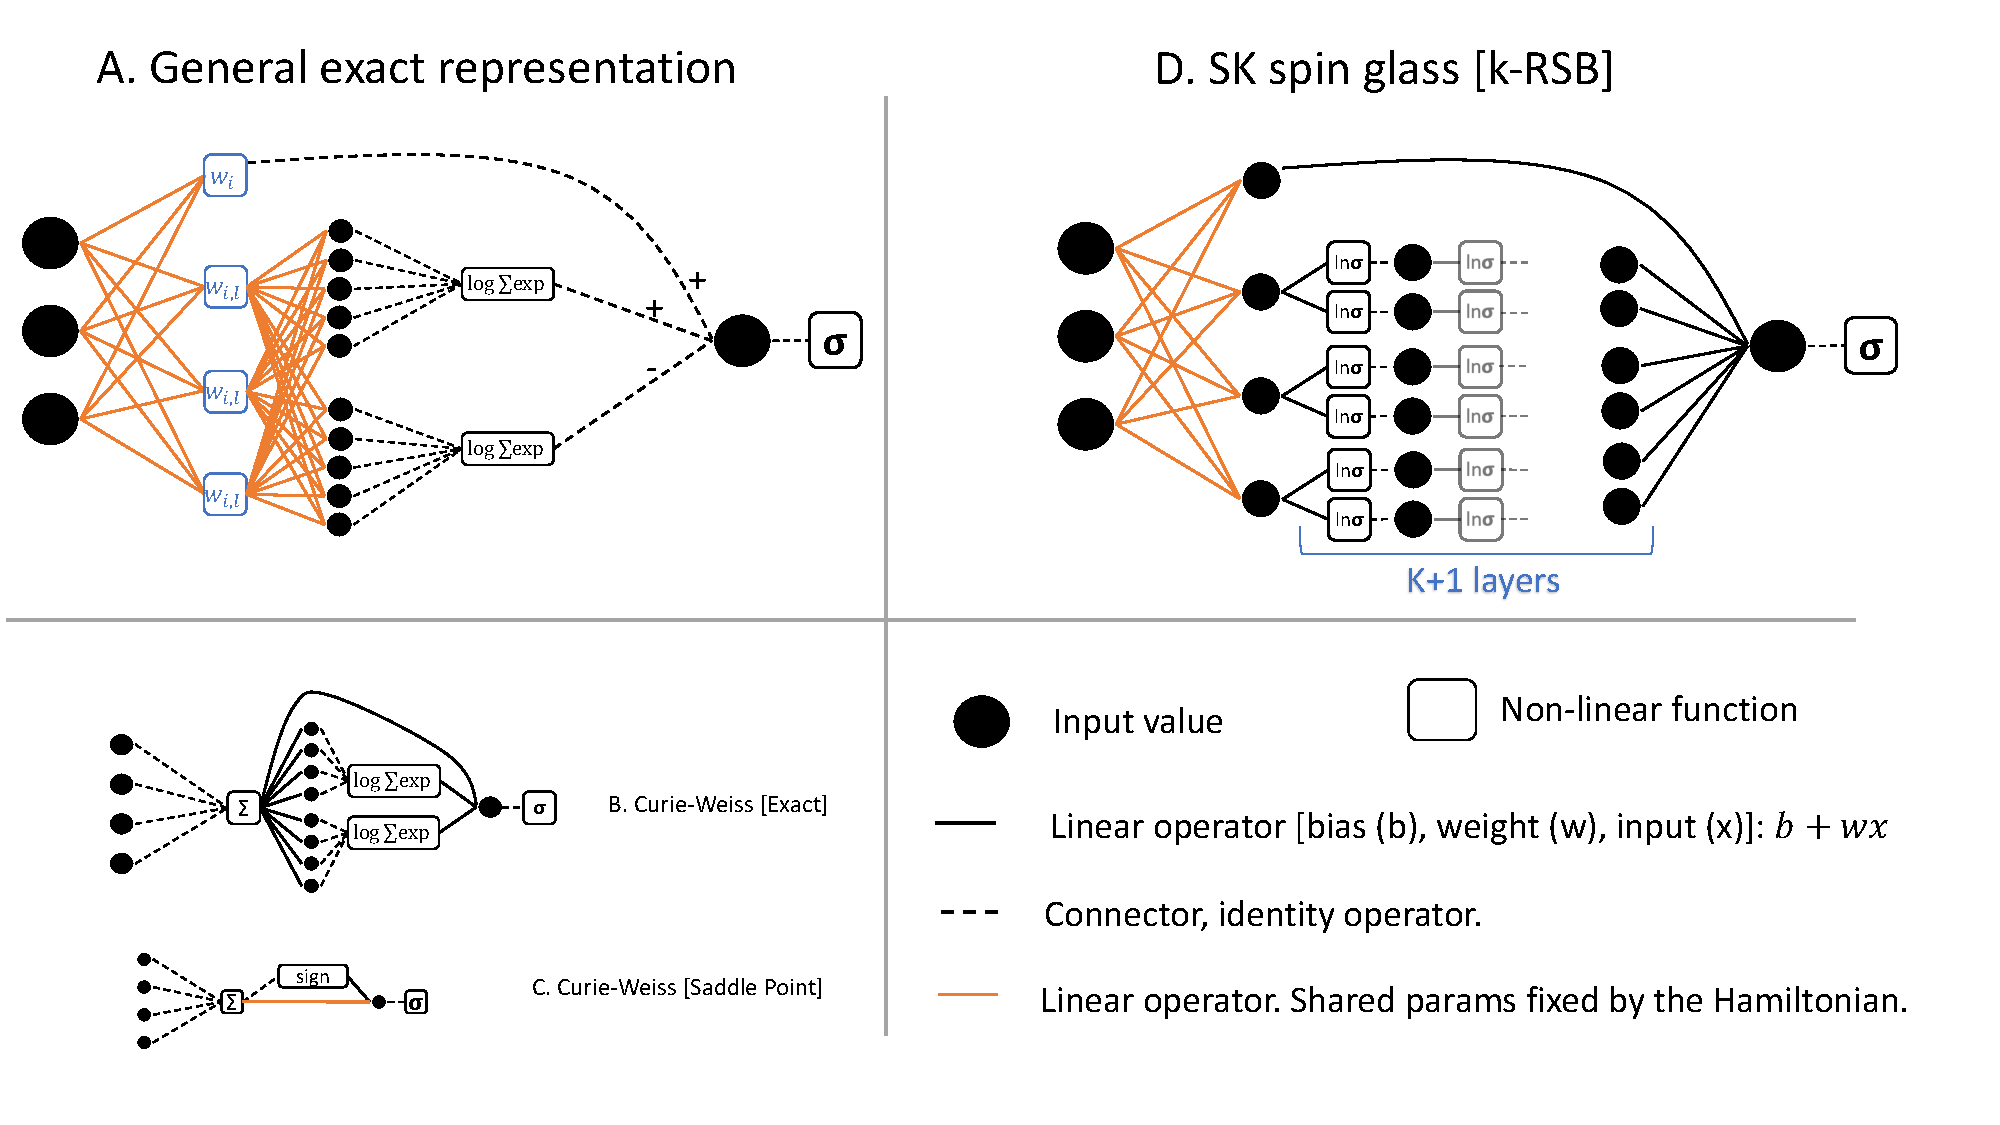
\includegraphics[width=0.5\textwidth]{img/ann_img.pdf}
    \caption{Neural network Architectures of conditional probability}
    \label{fig:arch_old}
\end{figure}

\section{Models}
\subsection{Curie-Weiss model}

The Curie-Weiss model (CW) is a uniform, fully-connected Ising model. Its Hamiltonian, with $N$ spins, is $H\left(\mathbf{x}\right)=-h\sum_{i=1}^{N}x_{i}-\frac{J}{N}\sum_{i<j}x_{i}x_{j}$. Defining $M_{<i}[\mathbf{x}_{<i}]=\sum_{s=1}^{i-1}x_{l}$ and $M_{>i}=\sum_{l=i+1}^{N}x_{l}$, the conditional probability of a spin $i$, eq.\ref{eq:conditional_ghann}, of the CW model is:
\begin{multline}
P^{CW}\left(x_{i}=1|\mathbf{x}_{<i}\right) = 
\sigma\bigg( 
 2 \beta h + 2 \beta \frac{J}{N}M_{i<}[\mathbf{x}_{<i}] + \\
 \log(\rho_i^+[\mathbf{x}_{<i}]) - \log(\rho_i^-[\mathbf{x}_{<i}])
\bigg),
\label{eq:conditional_cw}
\end{multline}
where:
\begin{equation}
\rho_i^{\pm}[\mathbf{x}_{<i}] \propto \sum_{\mathbf{x}_{>i}}e^{\beta \left(h\pm\frac{J}{N}+\frac{J}{N}M_{<i}[\mathbf{x}_{<i}]\right)M_{>i}+\frac{\beta J}{2N}M_{>i}^{2}} 
%\sum_{x_{i+1}\dots x_{N}} e^{\beta h_i^{\pm}[\mathbf{x}_{<i}]S_i +\frac{\beta J}{2N}S_{i}^{2}},
\label{eq:rho_cw_0}
\end{equation}
Defining $h_i^{\pm}[\mathbf{x}_{<i}] =h\pm\frac{J}{N}+\frac{J}{N}M_{<i}[\mathbf{x}_{<i}]$, at given $\mathbf{x}_{<i}$, the eq. \ref{eq:rho_cw_0} is equivalent to the partition function of CW model, with $N-i$ spins and external fields $h_i^{\pm}$. 
The sums over the configurations of the spins $l$ can be carried on easily:
\begin{multline}
 \rho_i^{\pm}[\mathbf{x}_{<i}] = \sum_{x_{i+1}\dots x_{N}} e^{\beta h_i^{\pm}[\mathbf{x}_{<i}]M_{>i} +\frac{\beta J}{2N}M_{>i}^{2}} \\
  = \sqrt{\frac{N}{2\pi \beta J}}\sum_{x_{i+1}\dots x_{N}}e^{\beta h_i^{\pm}[\mathbf{x}_{<i}] M_{>i}}\int e^{-\frac{N}{2J \beta}t^{2}+t M_{>i}} dt\\
  = \sqrt{\frac{N}{2\pi \beta J}}\int dt e^{-\frac{N}{2J \beta}t^{2}} \sum_{x_{i+1}\dots x_{N}}e^{(\beta h_i^{\pm}[\mathbf{x}_{<i}] + t) M_{>i}}  \\
 =  \sqrt{\frac{N}{2\pi \beta J}}\int dt e^{-\frac{N}{2J \beta}t^{2}} \left(e^{\beta h_i^{\pm}[\mathbf{x}_{<i}] + t} + e^{ (-\beta h_i^{\pm}[\mathbf{x}_{<i}] - t)} \right)^{N-i}  \\ 
 \label{eq:rho_last_exact}
 \end{multline} 
 where we used the Hubbard–Stratonovich (HS) transformation to obtain the second equality.\\
 First, in the following, we derive the exact feed-forward representation of eq.\ref{eq:conditional_cw} at finite $N$ number of variables, then in the limit to $N\rightarrow \infty$.\\

 \paragraph{Exact expression of the conditional probability of the CW model}
 The integral in the equation \ref{eq:rho_last_exact} can be computed the following way:

 \begin{eqnarray*}
 \rho_i^{\pm}[\mathbf{x}_{<i}] &=& \sqrt{\frac{N}{2\pi \beta J}}\int dt e^{-\frac{N}{2J \beta}t^{2}} 
 \sum_{k=0}^{N-i} \binom{N-i}{k} e^{(N-i-2k)*(\beta h_i^{\pm}[\mathbf{x}_{<i}] + t)}\\
 &=& \sum_{k=0}^{N-i} \binom{N-i}{k} \sqrt{\frac{N}{2\pi \beta J}}\int dt e^{-\frac{N}{2J \beta}t^{2}} 
  e^{(N-i-2k)*(\beta h_i^{\pm}[\mathbf{x}_{<i}] + t)}\\
&=& \sum_{k=0}^{N-i} \binom{N-i}{k}e^{\frac{\beta J}{2N}\left(N-i-2k\right)^{2}+\left(N-i-2k\right)\left(\beta h \pm \frac{\beta J}{N}\right)} e^{\frac{\beta J}{N}\left(N-i-2k\right) \sum_s x_s} \\
&=& \sum_{k=0}^{N-i} e^{a_{i,k}^{\pm} + b_{i,k}^{\pm} \sum_s x_s} 
\end{eqnarray*}
where we defined:
\begin{eqnarray}
\label{eq:params}
e^{b_{i,k}^{\pm}} & = & \binom{N-i}{k}e^{\frac{\beta J}{2N}\left(N-i-2k\right)^{2}+\left(N-i-2k\right)\left(\beta h \pm \frac{\beta J}{N}\right)}\\
e^{\omega_{i,k}^{\pm}} & = & e^{\frac{\beta J}{N}\left(N-i-2k\right)}.
\end{eqnarray}
The final feed-forward architecture of the Curie-Weiss Autoregressive Neural Network (CuWANN) architecture is:
\begin{multline}
\label{eq:curie_weiss_cond}
P^{CW}\left(x_{i}=+1|\mathbf{x}_{<i}\right)  =   \sigma \bigg[b_{i}+\omega_{i}\sum_{s=1}^{i-1}x_{s}\\
-\log\big(\sum_{k=0}^{N-i}e^{b_{i,k}^{+} + 
w_{i,k}^{+}\sum_{s=1}^{i-1}x_{s}}\big)+\log\big(\sum_{k=0}^{N-i}e^{b_{i,k}^{-} + w_{i,k}^{-}\sum_{s=1}^{i-1}x_{s}}\big)\bigg].
\end{multline}
where $b_i=2\beta h$ and $\omega_i=\frac{2\beta J}{N}$, see fig.\ref{fig:curie_weiss}. Their parameters have an analytic dependence from the parameters $J$ and $h$ of the Hamiltonian of the systems. 
%The set of parameters ($b_i, b_i^{k\pm}, \omega_i, \omega_i^{k\pm}$) can be consider as free parameters trained to minimize the KL divergence with the true probability distribution. 
It is interesting to note the number of parameters of the CuWANN is $2+4(N-i)$; they decrease as $i$ increases. This result is, somehow, the opposite of what the neural network architecture usually should take care of, meaning increasing the number of input variables, the number of parameters should also increase to describe the complexity of the function. Still, it is compatible with what was derived for the general case, where the number of parameters needed for the $\rho^{\pm}$ decreases exponentially with the index $i$. The CuWANN depends only on the sum of the input variables.
The total number of parameters of all conditional probability distribution scales as $2N^2+ O(N)$. 

\begin{figure}[!h]
    \centering
    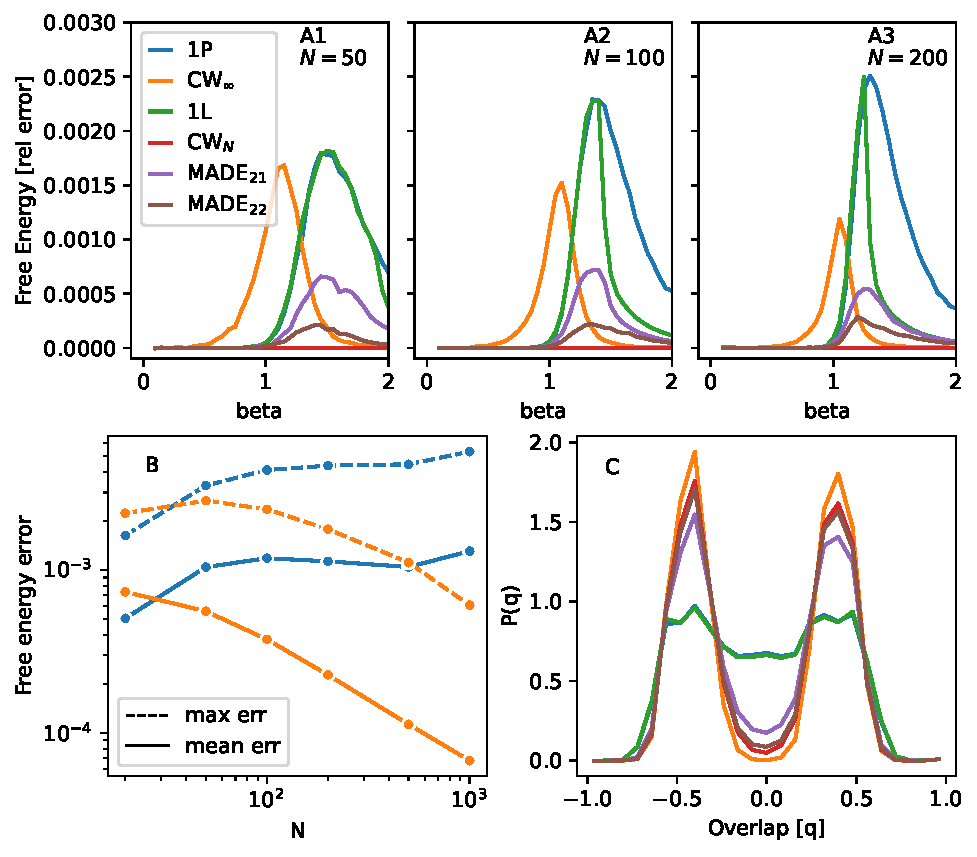
\includegraphics[width=0.5\textwidth]{img/CW_res.pdf}
    \caption{Results}
    \label{fig:curie_weiss}
\end{figure}


\paragraph{Saddle point method}
In the thermodynamical limit, the Curie-Weiss model admits an analytical solution. The order parameter of the system is the magnetization, $m_{\beta}=\frac{1}{N Z}\sum_{\mathbf{x}}\sum_i x_i e^{-\beta H}$ with $Z = \sum_{\mathbf{x}}\sum_i e^{-\beta H}$. At high temperature, with zero external fields $h=0$, the magnetization, $m_{\beta}$, is zero up to a critical temperature $\beta_c=1$, where a phase transition occurs, and a non-zero magnetization is observed. Considering the following variables: $\rho_i = \frac{N-i}{N}$, $m_i = -\frac{N-i-2k}{N}$, and for simplicity, the $h=0$ case, we can rewrite the expression, eq.\ref{eq:rho_last_exact}, as:
\begin{widetext}
    \begin{align*}
    \rho_i^{\pm}[\mathbf{x}_{<i}] &= \sqrt{\frac{N}{2\pi \beta J}}\int dt e^{-\frac{N}{2J \beta}t^{2}} 
    \sum_{k=0}^{N-i} \binom{N-i}{k} e^{(N-i-2k)*(\beta h_i^{\pm}[\mathbf{x}_{<i}] + t)}\\
    &= \sum_{k=0}^{N-i} \binom{N-i}{k}e^{\frac{\beta J}{2N}\left(N-i-2k\right)^{2}+\left(N-i-2k\right)\left(\pm\frac{\beta J}{N}\right)} e^{\frac{\beta J}{N}\left(N-i-2k\right) \sum_s x_s} \\
    &= \sum_{m_i=-\rho_i}^{\rho_i} \binom{N\rho_i}{\frac{N(m_i+\rho_i)}{2}} e^{\frac{N \beta J}{2}m_i^{2} \mp \beta J m_i } e^{N \rho_i \beta J \frac{\sum_s x_s}{N-i}}
    \end{align*}    
\end{widetext}

In the limit $N \gg 1$, and using the Stirling approximation for the binomial factor, we obtain:
 \begin{align}
 \rho_i^{\pm} & = 
  \int_{-\rho_i}^{\rho_i} \binom{N\rho_i}{\frac{N(m_i+\rho_i)}{2}} e^{\frac{N \beta J}{2}m_i^{2} \mp \beta J m_i } e^{N \rho_i \beta J \frac{\sum_s x_s}{N-i}} dm_i \\
\begin{split} 
  = & \int_{-\rho_i}^{\rho_i} \exp\bigg\{-N\rho\big( -\frac{1+\frac{m_i}{\rho_i}}{2} \log\frac{1+\frac{m_i}{\rho_i}}{2} \\
   & - \frac{1-\frac{m_i}{\rho_i}}{2} \log\frac{1-\frac{m_i}{\rho_i}}{2} 
      - \frac{\beta m_i^2}{2 \rho_i} + \beta m_i \frac{\sum_s x_s}{N-i}\big) \bigg\} e^{\mp \beta J m_i}
\end{split}
\end{align}
Solving the above integral using the saddle point method is possible by computing the extremes of the function inside the curly brackets. Deriving by $m_i$, we obtain that the extremes should satisfy the following equation:
\begin{equation}
\frac{m_i}{\rho_i} = \tanh \left( \beta(\frac{m_i}{\rho_i} - \frac{\sum_s x_s}{N-i}) \right)
\label{eq:extrem_i}
\end{equation}
In the $N$ large limit, and for a typical sample, we assume that: $\frac{\sum_s x_s}{N-i} \approx |\tilde{m}_{\beta}| \text{sign}(\sum_s x_s)$, where the $m_{\beta}$ is the magnetization of the Curie-Weiss system at inverse temperature $\beta$ and $\text{sign(x)} = \frac{|x|}{x}$ is the sign function.
We can distinguish two cases when the magnetization of the system is zero or not. 
In the first case, when $\beta\leq 1$, the solution of eq.\ref{eq:extrem_i} is zero as well, and $\log(\rho_i^{+}) - \log(\rho_i^{-})=0$ because the only term that makes the two quantities different, $\mp \beta J m_i$, vanish.\\ 
When instead the system acquires a magnetization $m_{\beta}$ different from zero, the eq.\ref{eq:extrem_i} admit one maximum that depends on the two possible symmetric values of $\frac{\sum_s x_s}{N-i}\approx |\tilde{m}_{\beta}| \text{sign}(\sum_q x_q)$. 
The solution of eq.\ref{eq:extrem_i}, $\pm \tilde{m}_{\text{extrem}}$ depends again on $\text{sign}(\sum_s x_s)$, and we can write the maximum solution as $\tilde{m}_{i}=|\tilde{m}_i| \text{sign}(\sum_s x_s)$. 
Easily we obtain that $\log(\rho_i^{+}) - \log(\rho_i^{-}) = -2\beta J|\tilde{m}_i| \text{sign}(\sum_s x_s)$. 
In the end, we can define the $\text{CuWANN}_{\infty}$ the following neural network architecture:
\begin{eqnarray}\
\label{eq:curie_weiss_cond2}
Q^{\Theta}\left(x_{i}=+1|\mathbf{x}_{<i}\right) & = & \sigma \left(b^0+\omega_{i}^0\sum_{s=1}^{i-1}x_{s} + \omega_i^1 \text{sign}(\sum_{s=1}^{i-1}x_{s})\right).
\end{eqnarray}
where $b^0=2\beta h$, $\omega^0_i = \frac{2\beta J}{N}$ are the same, and so shared, among all the conditional probability functions. The $\omega^1_i = -2\beta J |\tilde{m}_i|$ is different for each of them, and it will be set as free parameter to be learned during the training. The total number of parameters of the $\text{CuWANN}_{\infty}$ is $N+2$.

\subsection{spin glass}
The SK hamiltonian, with zero external fields for simplicity, is given by:
\begin{equation}
H\left(\mathbf{x}\right)=-\sum_{i<j}J_{ij}x_{i}x_{j}
\end{equation}
where the set of $\underline{J}$ are i.i.d. random variable extracted from a Gaussian probability distribution $P(J)=\sqrt{\frac{N}{2\pi}}\exp\left(\frac{-NJ^2}{2} \right)$. \\
To find a feed-forward representation of their conditional probability, we use the replica trick \cite{}. Usually, the replica trick is used in conjunction with the average over the system's disorder. In our case, we work with a single instance of the set of $Js$, but we assume that $N-i$ is large enough such that the following approximation is valid for the function $\rho_i$: 
\[
\log\rho_i^{\pm} \sim \mathbb{E}\left[  \log\rho_i^{\pm} \right] = \lim_{n\rightarrow 0} \frac{  \log(\mathbb{E}\left[(\rho_i^{\pm})^n \right])}{n}
\]
In the last equality, we use the replica trick. 
For each specific conditional probability, the average over the disorder $\mathbb{E}$ is taken on the coupling variables $J_{ll'}$ with $l,l'>i$. Implicitly, we assume that the quantities $\log\rho_i^{\pm}$ are a self-averaged quantity on the $\mathbf{x}_{i>}$ variables.
 The replica computation can be carried on easily, finding:
\begin{multline}
\mathbb{E}_{\underline{J}}\left[(\rho_i^{\pm}[\mathbf{x}_{<i}])^n \right]  = \\
\int \prod_{l<l'} dP_{J_{ll'}} \bigg\{ 
\sum_{\{\underline{x}^{a}\}_{i+1}^N} \exp\bigg[\beta \bigg(
\sum_{l,a}\bigg( \pm J_{il} + \sum_{s} J_{sl} x_s \bigg) x_l^{a} + \\
\sum_{l,l', a} J_{ll'} x_l^{a} x_{l'}^{a}
\bigg)  \bigg] 
\bigg\}\\
\end{multline}
where, the sums over $(l,l')$, $s$ and $a$ run respectively over $(i+1,N)$, $(1,i-1)$ and $(1,n)$, and $dP_{J_{ll'}}=P(J_{ll'})dJ_{ll'}$. We defined $h_l^{\pm}[\mathbf{x}_{<i}] =\pm J_{il} + \sum_{s=1}^{i-1} J_{sl} x_s$ and carrying out the integrals over the disorder variables $\{P(J_{ll'})\}$ yields:
\begin{widetext}
\begin{eqnarray}
\mathbb{E}_{\underline{J}}\left[(\rho_i^{\pm}[\mathbf{x}_{<i}])^n \right] & = & 
\sum_{\{\underline{x}^{a}\}_{i+1}^N} 
\exp\left\{\beta \left[
\sum_{l} h_l^{\pm}[\mathbf{x}_{<i}] \sum_{a} x_l^{a} +\frac{\beta}{2N} \sum_{l,l'} \sum_{a,b} x_l^{a} x_l^{b} x_{l'}^{a}x_{l'}^{b} \right]  \right\} \\
& = & e^{ \frac{(N-i) \beta^2}{4N}((N-i)n-n^2) } 
\sum_{\{\underline{x}^{a}\}_{i+1}^N} 
\exp\left\{\beta \left[
\sum_{l} h_l^{\pm}[\mathbf{x}_{<i}] \sum_{a} x_l^{a} +\frac{\beta}{2N} \sum_{a<b} \left( \sum_{l}  x_l^{a} x_l^{b} \right)^2 \right]  \right\}
\end{eqnarray}
\end{widetext}
Using the Hubbard-Stratonovich transformation of the quadratic terms, we can write:
\begin{widetext}
\begin{eqnarray}
\mathbb{E}_{\underline{J}}\left[(\rho_i^{\pm}[\mathbf{x}_{<i}])^n \right] & = & 
c(n,N,i)
\int \prod_{a<b} dQ_{ab} e^{-\frac{N}{2}\beta^2Q_{a,b}^2}
\sum_{\{\underline{x}^{a}\}_{i+1}^N} 
\exp\left\{\beta \left[
\sum_{l} h_l^{\pm}[\mathbf{x}_{<i}] \sum_{a} x_l^{a} +\beta \sum_{a<b} Q_{a,b} \sum_{l}  x_l^{a} x_l^{b} \right]  \right\} \\
& = & 
c(n,N,i)
\int \prod_{a<b} dQ_{ab} e^{-\frac{N}{2}\beta^2Q_{a,b}^2}
\prod_{l} \left[
\sum_{\{\underline{x}^{a}_l\}} 
\exp\left\{\beta \left[
h_l^{\pm}[\mathbf{x}_{<i}] \sum_{a} x_l^{a} +\beta \sum_{a<b} Q_{a,b}  x_l^{a} x_l^{b} \right]  \right\}
\right] \label{eq:before_ansaltz}
\end{eqnarray}
\end{widetext}
where we defined: 
$$c(n,N,i) = e^{ \frac{(N-i) \beta^2}{4N}((N-i)n-n^2) } \left(\frac{2\pi \beta^2}{N}\right)^{\frac{n(n-1)}{2}}.$$ 
The celebrated \cite{pippo2021} Parisi solutions of the SK model prescribe how to parametrize the matrix of the overlaps $Q$ \cite{10.1142/0271}. The following shows how to obtain neural network architectures based on the replica symmetric (RS) and k-step replica symmetric broken (k-RSB) solutions.

\begin{figure}[]
    \centering 
    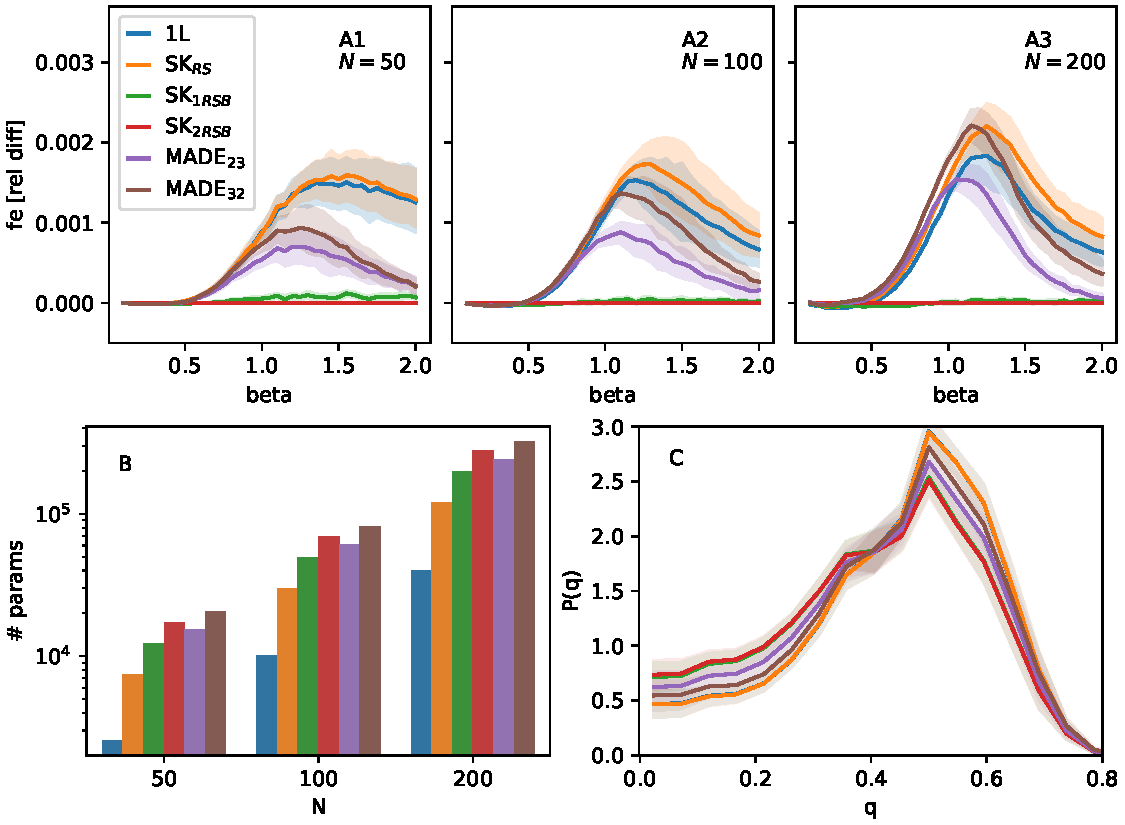
\includegraphics[width=0.5\textwidth]{img/SK_res.pdf}
    \caption{Results}
    \label{fig:SK}
\end{figure}


\subsubsection{Replica Symmetric solution (RS)}
We assume that the overlaps between the replicas are symmetric under permutations, and the matrix of the overlaps between replicas is parametrized with only one variable $q$:
$$
Q_{a,b}=\begin{cases}
			0, & \text{if $a=b$}\\
            q, & \text{otherwise}
		 \end{cases},
$$
obtaining:
\begin{widetext}
\begin{eqnarray}
\mathbb{E}_{\underline{J}}\left[(\rho_i^{\pm, sym}[\mathbf{x}_{<i}])^n \right] & = & 
c(n,N,i)
\int dq e^{-\frac{n(n-1)N}{4}\beta^2 q^2}
\prod_{l} \left[
\sum_{\{\underline{x}^{a}_l\}} 
\exp\left\{\beta \left[
h_l^{\pm}[\mathbf{x}_{<i}] \sum_{a} x_l^{a} +\beta q \sum_{a<b} x_l^{a} x_l^{b} \right]  \right\} 
\right] \\
& = &
c(n,N,i)
\int dq e^{-\frac{n(n-1)N}{4}\beta^2 q^2}
e^{-\frac{nN\beta^2 q}{2}}
\prod_{l} \left[
\sum_{\{\underline{x}^{a}_l\}} 
e^{\beta \left[
h_l^{\pm}[\mathbf{x}_{<i}] \sum_{a} x_l^{a} + \frac{\beta q}{2} \left(\sum_{a} x_l^{a} \right)^2 \right]} 
\right]\\
& = &
c'(n,N,i)
\int dq e^{-\frac{n(n-1)N}{4}\beta^2 q^2}
e^{-\frac{nN\beta^2 q}{2}}
\prod_{l} \left[\int \frac{dz_l}{\sqrt{2\pi q}} e^{-\frac{z_l^2}{q}}
\sum_{\{\underline{x}^{a}_l\}} 
e^{\beta \left(
h_l^{\pm}[\mathbf{x}_{<i}] +\beta z_l \right) \sum_{a} x_l^{a}} 
\right]\\
& = &
c'(n,N,i)
\int dq e^{-nN\left(\frac{(n-1)}{4}\beta^2 q^2 +\frac{\beta^2 q}{2}\right)}
\prod_{l} \left[\int \frac{dz_l}{\sqrt{2\pi q}} e^{-\frac{z_l^2}{q}}
2^n\cosh^n \left(\beta \left(
h_l^{\pm}[\mathbf{x}_{<i}] +\beta z_l \right)\right) 
\right].\\
\end{eqnarray}
\end{widetext}
Using the limit that $n\rightarrow 0$ we can write:
\begin{widetext}
\begin{eqnarray}
\int \frac{dz_l}{\sqrt{2\pi q}} e^{-\frac{z_l^2}{q}}
2^n\cosh^n \left(\beta \left(
h_l^{\pm}[\mathbf{x}_{<i}] +\beta z_l \right)\right) = e^{n \int \frac{dz_l}{\sqrt{2\pi q}} e^{-\frac{z_l^2}{q}}
\log 2\cosh \left(\beta \left(
h_l^{\pm}[\mathbf{x}_{<i}] +\beta z_l \right)\right)}.
\label{eq:gauss_n0}
\end{eqnarray}
\end{widetext}
obtaining:
\begin{widetext}
\begin{eqnarray}
\log (\rho_i^{\pm, sym}[\mathbf{x}_{<i}]) & = & 
\lim_{n\rightarrow 0} \frac{1}{n} \log \left( c'(n,N,i)
\int dq e^{-\frac{n(n-1)N}{4}\beta^2 q^2}
e^{-\frac{nN\beta^2 q}{2}}
e^{n \sum_l 
\int \frac{dz_l}{\sqrt{2\pi q}} e^{-\frac{z_l^2}{q}}
\log 2\cosh \left(\beta \left(
h_l^{\pm}[\mathbf{x}_{<i}] +\beta z_l \right)\right)
} 
\right)\\
& = &
\log(c''(N,i)) + 
\left( +\frac{N}{4}\beta^2 q^2_0 
-\frac{N\beta^2 q_0}{2}
+ \sum_l 
\int \frac{dz_l}{\sqrt{2\pi q_0}} e^{-\frac{z_l^2}{q_0}}
\log 2\cosh \left(\beta \left(
h_l^{\pm}[\mathbf{x}_{<i}] +\beta z_l \right)\right)
\right) \\
& \doteq &  
c(N,i, q_0) -
\sum_l 
\int \frac{dz_l}{\sqrt{2\pi q_0}} e^{-\frac{z_l^2}{q_0}}
\log \sigma \left(\beta \left(
2h_l^{\pm}[\mathbf{x}_{<i}] +2\beta z_l \right)\right)
\end{eqnarray}
\end{widetext}
In the second line we use the saddle point methods to evaluate the integral over $q$, assuming that the single maximum value $q_0$ does not depend on the input values $\mathbf{x}_{<i}$ in the set of $h_l^{\pm}[\mathbf{x}_{<i}]$. It is a bold assumption to be verified {\it a posteriori} on the goodness of the neural network architectures performances. 
In the third line, we use the identity $\log\cosh(x) = 2x - \log\sigma(2x)$ and the elements that are equals between $\log(\rho^+)$ and $\log(\rho^-)$ are simplified. We introduced the $\log\sigma$ non-linear operator for computational reason.

% We can, after some manipulations, obtain a more neural network friendly function:
% \begin{eqnarray}
% \log (\rho_i^{\pm, sym} [\underline{x_l}])^n] & \approx & 
% \text{Extr}_q \left( +\frac{N}{4}\beta^2 q^2 
% -\frac{N\beta^2 q}{2}
% + \sum_l 
% \int dz_l e^{-z_l^2}
% \log \cosh \left(\beta \left(
% h_l +\beta \sqrt{q}z_l \right)\right)
% \right) 
% \end{eqnarray}

Now we consider the following approximation of the Gaussian convolution:
\[
\int dz e^{-z^2}
\log \sigma \left(\beta \left(
h +\beta \sqrt{q}z \right)\right) \sim b_0 + w_0*\log \sigma(b_1 + w_1 h), 
\]
where $(b_0, w_0, b_1,w_1)$ are free parameters to be determined. In Supporting Material (SI) a numerical analysis of the correctness of this approximation is shown.  
Putting together all the pieces, we can parameterize the conditional probability as:
\begin{multline}
Q^{RS}\left(x_{i}=1|\mathbf{x}_{<i}\right) = \sigma\left( 
    x_i^1(\mathbf{x}_{<i}) +\log(\rho_i^+) - \log(\rho_i^-)
\right) \\
 = \sigma \bigg( x_i^1(\mathbf{x}_{<i}) + \sum_{l^+=i+1}^{N}  w_0^{i,l^+} \log\sigma(b_1^{i,l^+} +
 w_1^{i,l^+} x_{i,l^+}^1(\mathbf{x}_{<i}))+ \\
 + \sum_{l^-=i+1}^{N}  w_0^{i,l^-} \log\sigma(b_1^{i,l^-} + w_1^{i,l^-} x_{i,l^-}^1(\mathbf{x}_{<i})
 \bigg) 
\end{multline}
where the set of $(\mathbf{b},\mathbf{w})$ are free variational parameters to learn. 
%The $\sum_l$ considers all the elements together of the plus and minus $\rho^{\pm}$ function. 
\\DO the image of the nets.


\subsubsection{K-step Replica symmetric breaking (k-RSB)}
Assuming that the replica symmetry is broken, we can use the following ansatz called 1-step replica symmetric breaking (1RSB), where the overlaps between replicas are divided into $m$ blocks:
\begin{eqnarray}
    Q_{a,b}=\begin{cases}
			q_1, & \text{if } I(a/m)=I(b/m) \\
            q_0. & \text{if } I(a/m) \neq I(b/m).
		 \end{cases}
\end{eqnarray}
With the above ansatz, we can compute the following quantities:
\begin{align}
\begin{split}
    \sum_{ab} Q_{ab} x_{a} x_{b}  &  = \frac{1}{2} \bigg[ q_0 \left( \sum_{a}x_a\right)^2 +\\ 
& (q_1-q_0) \sum_{\text{blocks}}  \left( \sum_{a \in \text{block}}x_a\right)^2   - nq_1\bigg] 
\end{split}
\\
\sum_{ab} Q_{ab}^2 & =  n^2 q_0^2 + nm(q_1^2 - q_0^2) -n q_1^2.
\end{align}
The equation \ref{eq:before_ansaltz} becomes:
\begin{widetext}
\begin{align}
& \mathbb{E}_{\underline{J}} \left[(\rho_i^{\pm, 1RSB})^n \right] =  \\[1ex]
\begin{split}
& = c(n,N,i) \int dq_1 dq_0 e^{\frac{N}{2}\beta^2 \left[n^2 q_0^2 + nm(q_1^2 - q_0^2) -n q_1^2 \right]} 
\prod_{l} \bigg[ \sum_{\{\underline{x}^{a}_l\}} e^{ \beta \big[ h_l^{\pm} \sum_{a} x_l^{a} +\beta q_0 \left( \sum_{a} x_p^{a} \right)^2 + \beta (q_1-q_0) \sum_{\text{blocks}} \left( \sum_{a \in \text{block}}x_l^{a}\right)^2  -n q_1 \bigl]}  \bigg] 
\end{split}\\ 
\begin{split}
& = c(n,N,i) \int dq_1 dq_0 e^{\frac{N}{2}\beta ^ 2 \left[n^2 q_0^2 + nm(q_1^2 - q_0^2) -n q_1^2 -n q_1\right]} 
\prod_{l} \bigg[ \sum_{\{\underline{x}^{a}_l\}} \int dP_{z_l} \prod_{k=1}^{n/m} \int dP{y_{lk}}  e^{\beta \big[h_l^{\pm} \sum_{a} x_l^{a} + \beta z_l \sum_{a}x_l^{a} + \beta \sum_{\text{blocks}}  y_{lk} \sum_{a \in \text{block}}x_l^{a}\bigl]}  \bigg] 
\end{split}\\ 
\begin{split}
& = c(n,N,i) \int dq_1 dq_0 e^{\frac{N}{2}\beta^2 \left[n^2 q_0^2 + nm(q_1^2 - q_0^2) -n q_1^2 -n q_1\right]} 
\prod_{l} \bigg[ \int dP_{z_l}  \prod_{k=1}^{n/m} \int dP_{y_{lk}} \cosh^m\bigg(\beta \big[h_l^{\pm}+ \beta z_l +\beta y_{lk}\bigl]  \bigg)  \bigg]
\end{split}\\ 
\begin{split}
& = c'(n,N,i) + c(n,N,i) \int dq_1 dq_0 e^{\frac{N}{2}\beta\left[n^2 q_0^2 + nm(q_1^2 - q_0^2) -n q_1^2 -n q_1\right]} 
\prod_{p} \int dP_{z_l}  \exp \bigg\{ \frac{n}{m} \log \bigg( \int dP_{y_{l}} \cosh^m\bigg(\beta \big[h_l^{\pm}+ \beta z_l + \beta y_{l}\bigl]  \bigg)  \bigg) \bigg\},
\end{split}\\ 
\end{align}
\end{widetext}
where we defined:
\begin{align}
    dP_{z_l} & = \frac{dz_l}{\sqrt{2\pi q_0}}e^{\frac{z^2}{2q_0}}\\
    dP_{y_{l}} & = \frac{dy_{l}}{\sqrt{2\pi (q_1-q_0)}}e^{\frac{y_{l}^2}{2 (q_1-q_0)}}.
\end{align}
Considering $N \gg 1$ and $n\rightarrow 0$ to use the saddle point methods and the identity in eq.\ref{eq:gauss_n0}, we can write:
\begin{widetext}
\begin{align}
\log (\rho_i^{\pm, 1RSB}) & = 
\lim_{n\rightarrow 0} \frac{1}{n} \log \left(\mathbb{E}_{\underline{J}} \left[(\rho_i^{\pm, 1RSB})^n \right]  \right) \\
& = c_i +  \text{Extr}_{q_0, q_1} \bigg[ c'_i(N,n,q_0, q_1) 
+ \frac{1}{m} \sum_{l} \int dP_{z_l} \log \bigg( \int dP_{y_{l}} \cosh^m\bigg(\beta \big[h_l^{\pm}+ \beta z_l + \beta y_{l}\big]  \bigg)  \bigg)
\bigg].
\end{align}
\end{widetext}

The above integrals are rewritten as the following:
\begin{align}
& \int dP_{z_l} \log \bigg( \int dP_{y_{l}}  \cosh^m\bigg(\beta \big[h_l^{\pm}+\beta z_l + \beta  y_{l}\big]  \bigg)  \bigg) 
 = \\
& \int dP_{z_l} \log \biggl( \int dP_{y_{l}} e^{ m \log \cosh \left(\beta \left[h_l^{\pm}+ \beta  z_l + \beta  y_{l}\right]  \right) } \biggr) 
 = \\
& \beta h_{l}^{\pm} + \int dP_{z_l} \log \biggl( \int dP_{y_{l}} e^{\beta^2 m y_{l} - m \log \sigma \left(\beta \left[h_l^{\pm}+ \beta z_l +\beta y_{l}\right]  \right) } \biggr) 
\end{align}
We have two nested gaussian convolutions. In order to make it easier to compute this non-linear operator, we will use a sequence of approximations similar to those used previously for RS case. %Recalling $h_l^{\pm}[\mathbf{x}_{<i}] =\pm J_{il} + \sum_{s} J_{sl} x_s$, we consider the approximation of the nested gaussian convolution:
%\begin{multline}
%f(\mathbf{x}_{<i}) = \int \frac{dz_l}{\sqrt{2\pi q_0}}e^{\frac{z^2}{2q_0}} \log \bigg( \int \frac{dy_{l}}{\sqrt{2\pi (q_1-q_0)}}e^{\frac{y_{l}^2}{2 (q_i-q_0)}} \\
% e^{ y_{l} - m \log \sigma \left(\beta \left[\pm J_{il} + \sum_{s} J_{sl} x_s + h + z_l + y_{l}\right]  \right) } \bigg) 
%\end{multline}
%Fixed the parameters of the model $(\{J_{pq}\}, h, \beta)$, this is a function that depends from three free parameters $(q_0, q_1, m)$. 
The integrals concerning the variables $(z_l, y_l)$ are approximated in the same way as the approach used previously for RS case: The number of free parameters increases to have feed-forward functions without integrals. First, we consider the following maps:
\begin{widetext}
\begin{align}
        & \int dP_{z_l}  \log \int dP_{y_{l}} e^{ \beta^2 m y_{l} - m \log \sigma \left(\beta \left[h_l^{\pm}+ z_l + y_{l}\right]  \right) }  \approx\\
        & \int dP_{z_l} \log \bigg( e^{\hat{b}_0^{l^{\pm}}}(1 + e^{\hat{b}_1^{l^{\pm}} + \hat{w}_1^{l^{\pm}} \log \sigma (\hat{b}_2^{l^{\pm}} + \hat{w}_2^{l^{\pm}} (h_l^{\pm}+ z_l)) }) \bigg) = \\
        & \hat{b}_0^{l^{\pm}} + \hat{w}_0^{l^{\pm}} \int dP_{z_l} \log \sigma \bigg(\hat{b}_1^{l^{\pm}} + \hat{w}_1^{l^{\pm}} \log \sigma (\hat{b}_2^{l^{\pm}} + \hat{w}_2^{l^{\pm}} (h_l^{\pm}+ z_l)) \bigg) \approx \\
        & b_0^{l^{\pm}} + w_0^{l^{\pm}} \log \sigma (b_1^{l^{\pm}} + w_1^{l^{\pm}} \log \sigma (b_2^{l^{\pm}} + w_2^{l^{\pm}} (h_l^{\pm}))),
%        \int dx e^{\frac{x^2}{a}} \log\sigma (a_1 + b_1 \log \sigma (a_2 + b_2 (h+x))) & \approx a_0 +b_0 \log \sigma (a'_1 + b'_1 \log \sigma (a'_2 + b'_2 (h))) 
\end{align}
\end{widetext}
where the set of parameters $(\mathbf{b_0^{{\pm}}},\mathbf{w_0^{{\pm}}},\mathbf{b_1^{{\pm}}},\mathbf{w_1^{{\pm}}},\mathbf{b_2^{{\pm}}},\mathbf{w_2^{{\pm}}})$ are free parameters to be determined by the learning procedures. The gaussian convolution integrals are substituted by feed-forward non-linear operations, enlarging the space of parameters. For the 1RSB case, we use the following architecture:
\begin{widetext}
\begin{multline}
    Q^{1RSB}\left(x_{i}=1|\mathbf{x}_{<i}\right) = \sigma\left( 
        x_i^1(\mathbf{x}_{<i}) +\log(\rho_i^+) - \log(\rho_i^-)
    \right) 
     = \sigma \bigg( x_i^1(\mathbf{x}_{<i}) + \\ \sum_{l^+=i+1}^{N}  w_0^{i,l^+} \log\sigma(b_1^{i,l^+} + 
     w_1^{i,l^+} \log\sigma(b_2^{i,l^+} +
     w_2^{i,l^+}  x_{i,l^+}^1(\mathbf{x}_{<i})))+ \sum_{l^-=i+1}^{N}  w_0^{i,l^-} \log\sigma(b_1^{i,l^-} + w_1^{i,l^-} \log\sigma(b_2^{i,l^+} +
     w_2^{i,l^+} x_{i,l^-}^1(\mathbf{x}_{<i})))
     \bigg) 
\end{multline}   
\end{widetext}
The generalization of the $\rho$ parametrization to the K-RSB case is straightforward. For instance for 2-RSB we have:
\begin{multline}
    \log \rho^{\pm, 2RSB} \left(x_{i}=1|\mathbf{x}_{<i}\right)  =  
   \sum_{l^{\pm}} w_0^{i,l^{\pm}} \log\sigma(b_1^{i,l^{\pm}} +\\
   w_1^{i,l^{\pm}} \log\sigma(b_2^{i,l^{\pm}} +
    w_2^{i,l^{\pm}}( \log\sigma(b_3^{i,l^{\pm}} +
    w_3^{i,l^{\pm}}x_{i,l^{\pm}}^1(\mathbf{x}_{<i})))))
\end{multline}

\section{Numerical evidence of Gaussian convolution approximations}

The case of replica:
\[
 \int dt e^{-\frac{Nt^2}{2K}}\log\cosh(K*h+t) \approx \left(\sum_{t \in \text{Extrem}^+}  b_i^t + c_i^t\log\cosh(d_i^t+e_i^t h)\right)
\label{eq:CW_gauss_approx2}
\]

\begin{figure}[h]
    \centering
    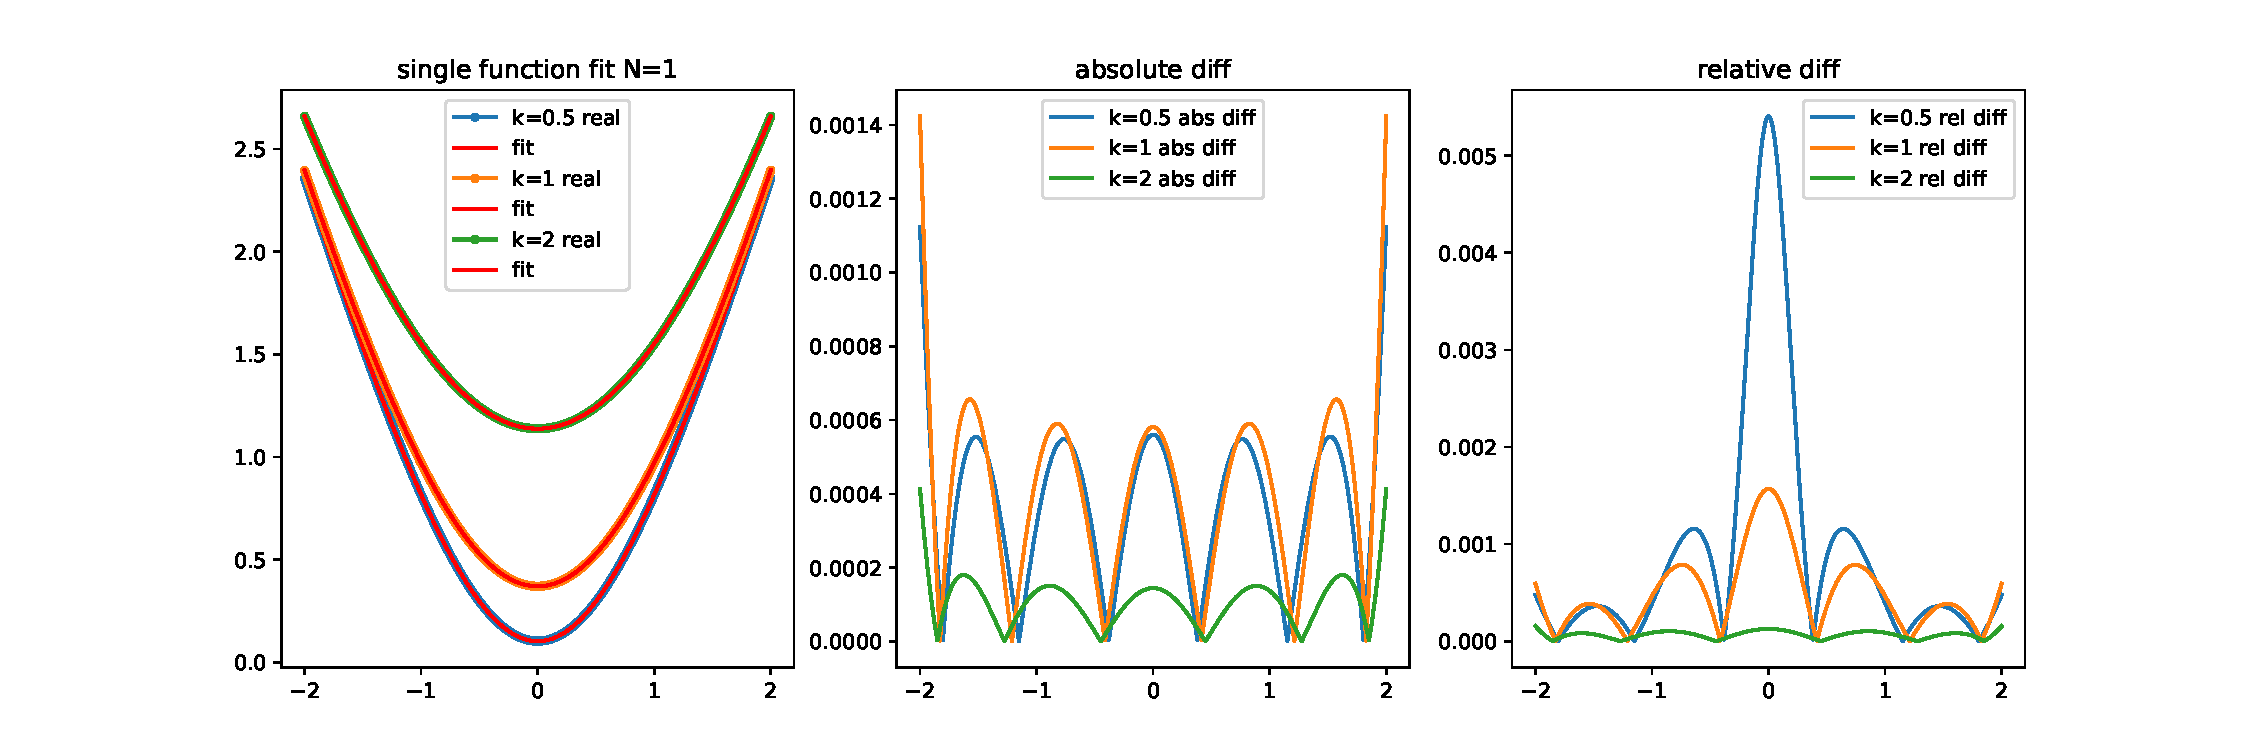
\includegraphics[width=1\textwidth]{img/RFIM_fit.pdf}
    \caption{Fit of eq.\ref{eq:CW_gauss_approx} at different values of $K=J\beta$. In the first row only one extreme is considered and two in the second row.}
    \label{fig:gauss_approx}
\end{figure}

\bibliography{refs}% Produces the bibliography via BibTeX.

\end{document}
  